\documentclass[preprint]{elsarticle}
\usepackage{hyperref}
\usepackage{amsmath}
\usepackage{url}
\usepackage[spanish]{babel}
\usepackage[utf8]{inputenc}
\usepackage{graphicx}
\usepackage{float}


\bibliographystyle{model2-names}


\begin{document}

\begin{frontmatter}

\title{Comportamiento de algunos mapas logísticos acoplados}


\author[md]{Marcos Daniel Calderón-Calderón}



\address[md]{Center for Research in Mathematics (CIMAT), Guanajuato, México.}


\begin{abstract}
En este documento, se presenta un pequeño reporte sobre el comportamiento de algunos mapas logísticos acoplados.
\end{abstract}



\end{frontmatter}



 
   
 
 


\section*{Introducción}
El mapa logístico en su forma discreta, presenta la siguiente forma:

\begin{equation}
X_{n+1}= \lambda X_{n}(1 - X_{n})
\end{equation}
donde $\lambda$ es un parámetro que debe tomar valores muy cercanos a 4 para que la seguencia presente buenas propiedades caóticas.


\section*{Partición del intervalo [0,1)}
A continuación, la tabla~\ref{tabo} muestra las particiones del intervalo donde el mapa logístico puede tomar valores.




\begin{table}[H]
\centering
\scalebox{0.9}{
\begin{tabular}{lllll}
\hline   
\textbf{Parte 1} & \textbf{Parte 2} & \textbf{Parte 3}  & \textbf{Parte 4}   & \textbf{Parte 5}   \\        
\hline
 0.010000   &      0.210000     &  0.410000      & 0.610000   &   0.810000   \\
 0.020000   &      0.220000     &  0.420000     & 0.620000   &    0.820000   \\
 0.030000   &     0.230000      &  0.430000      & 0.630000   &   0.830000   \\ 
 0.040000   &     0.240000      & 0.440000     & 0.640000    &    0.840000   \\
 0.050000   &      0.250000     & 0.450000       & 0.650000   &   0.850000   \\
 0.060000   &     0.260000      & 0.460000      & 0.660000   &    0.860000   \\
 0.070000   &      0.270000     & 0.470000      & 0.670000    &   0.870000     \\  
 0.080000   &     0.280000      &  0.480000     & 0.680000    &    0.880000     \\
 0.090000   &       0.290000    & 0.490000       & 0.690000    &    0.890000     \\
 0.100000   &       0.300000    &  0.500000      & 0.700000   &     0.900000     \\
 0.110000   &       0.310000    & 0.510000      & 0.710000    &     0.910000     \\
 0.120000   &     0.320000      & 0.520000     & 0.720000    &      0.920000     \\
 0.130000   &       0.330000    & 0.530000      & 0.730000    &     0.930000     \\
 0.140000   &      0.340000     & 0.540000     & 0.740000    &      0.940000    \\
 0.150000   &       0.350000    & 0.550000       & 0.750000    &    0.950000     \\
 0.160000   &      0.360000     & 0.560000       & 0.760000    &  0.960000    \\
 0.170000   &       0.370000    & 0.570000       & 0.770000    &   0.970000     \\
 0.180000   &      0.380000     &  0.580000     & 0.780000    &    0.980000   \\
 0.19000    &      0.390000     &  0.590000     & 0.790000    &   0.990000     \\
 0.20000    &       0.400000    & 0.600000     &   0.800000   &   1.000000  \\
\hline
\end{tabular}
}
\caption{Particiones utilizadas.}
\label{tabo}
\end{table}




\section{Esquema 1: \textbf{Ocho mapas acoplados sin la operación XOR} en secuencia de salida}
\label{esq1}

En este esquema, se utilizan ocho mapas acoplados; sin embargo, no existe una operación XOR en los valores de salida. Además, todas las $\lambda$'s  fueron inicializadas con el valor 3.9999. 

A continuación, se muestra una tabla de los parámetros y valores iniciales para cada uno de los mapas.

\begin{table}[H]
\centering
\scalebox{0.9}{
\begin{tabular}{lllll}
\hline   
\textbf{Mapa} & \textbf{Valor} & \textbf{Parámetro} \\
             & \textbf{Inicial} & \textbf{Utilizado} \\
\hline
\textit{Mapa 1}    & 	0.00345            &  3.9999    \\
\textit{Mapa 2}    & 	0.00021            &	  3.9999    \\
\textit{Mapa 3}    & 	0.00056            &	  3.9999    \\
\textit{Mapa 4}    & 	0.0006543          &	  3.9999    \\
\textit{Mapa 5}    & 	0.0005433          &	  3.9999    \\
\textit{Mapa 6}    & 	0.0003497          &	  3.9999    \\
\textit{Mapa 7}    & 	0.00561            &	  3.9999    \\
\textit{Mapa 8}    & 	0.0007670          &	  3.9999   \\
\hline
\end{tabular}
}
\caption{Valores para cada uno de los mapas utilizados en el esquema 1.}
\label{table1}
\end{table}

A continuación figura~\ref{f1} se muestra una gráfica de frecuencias de los datos generados por el sistema de mapas logísticos acoplados, se ha dividido el intervalo $[0,1)$ en 100 particiones, cada valor generado es clasificado en alguna de las particiones.

\begin{figure}[H]  
\centering
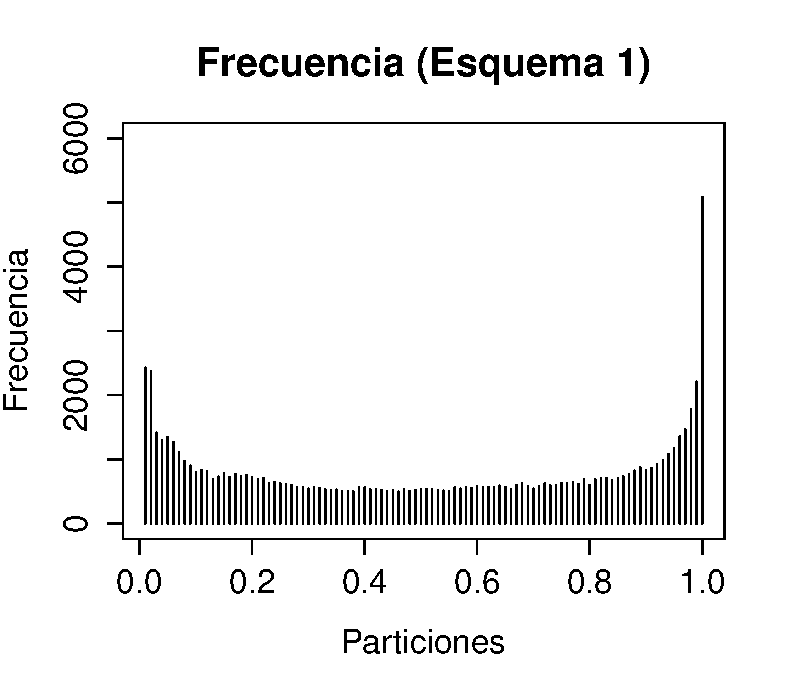
\includegraphics[width=8cm]{figure1.pdf}
\caption{Histograma de los valores generados en el esquema 1.}
\label{f1}
\end{figure}


Ahora, en la figura~\ref{f2} se muestra la distribución de los datos generados. Se debe de recordar que estos datos se generan cuando se multiplican los valores obtenidos de las mapas logísticos acoplados con el máximo valor que puede ser almacenado en un tipo de dato formado por 32 bits.

\begin{figure}[H]
\centering
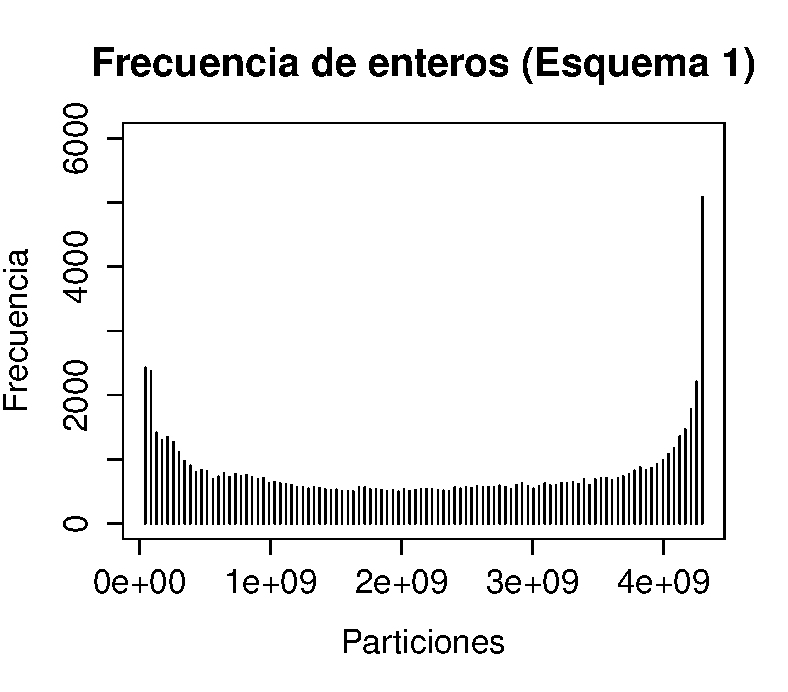
\includegraphics[width=8cm]{figure2.pdf}
\caption{Histograma de valores caóticos discretizados para el esquema 1.}
\label{f2}
\end{figure}



\section{Esquema 2: \textbf{Ocho mapas acoplados con la operación XOR} en secuencia de salida}
\label{esq2}

En este esquema hay una variación, a la hora de hacer la discretización de los valores obtenidos, se aplica una operación XOR secuencial. A continuación, se observa la tabla~\ref{table2} que muestra los parámetros utilizados en este ejemplo.

\begin{table}[H]
\centering
\scalebox{0.9}{
\begin{tabular}{lllll}
\hline   
\textbf{Mapa} & \textbf{Valor} & \textbf{Parámetro} \\
             & \textbf{Inicial} & \textbf{Utilizado} \\
\hline
\textit{Mapa 1}    & 	0.34561       &  3.9999    \\
\textit{Mapa 2}    & 	0.98687           &	  3.9999    \\
\textit{Mapa 3}    & 	0.54735            &	  3.9999    \\
\textit{Mapa 4}    & 	0.04576          &	  3.9999    \\
\textit{Mapa 5}    & 	0.94584          &	  3.9999    \\
\textit{Mapa 6}    & 	0.78594          &	  3.9999    \\
\textit{Mapa 7}    & 	0.62384            &	  3.9999    \\
\textit{Mapa 8}    & 	0.86560          &	  3.9999   \\
\hline
\end{tabular}
}
\caption{Valores para cada uno de los mapas utilizados en el esquema 2.}
\label{table2}
\end{table}


A continuación figura~\ref{f3} se muestra una gráfica de frecuencias de los datos generados por el sistema de mapas logísticos acoplados con operación XOR secuencial, se ha dividido el intervalo $[0,1)$ en 100 particiones, cada valor generado es clasificado en alguna de las particiones.


\begin{figure}[H]  
\centering
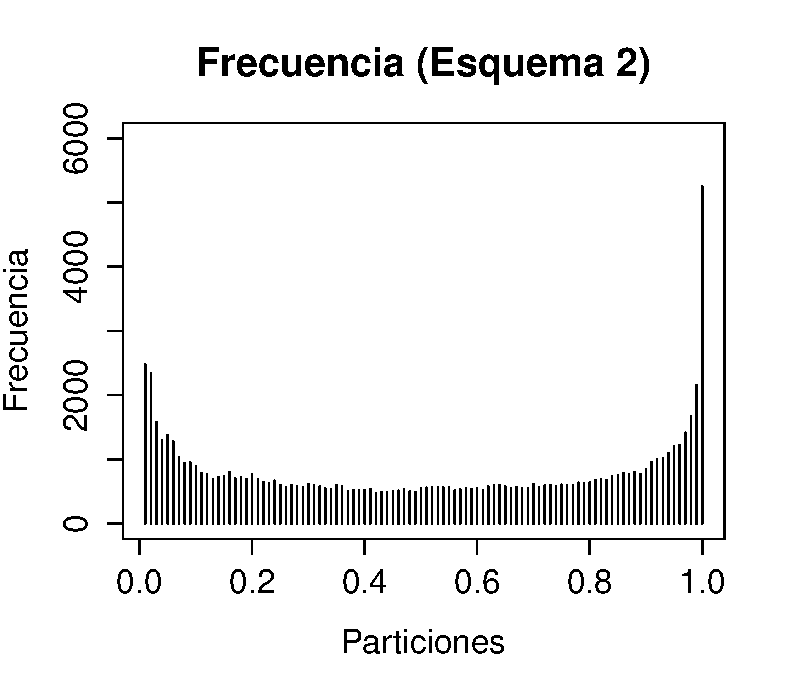
\includegraphics[width=8cm]{figure3.pdf}
\caption{Histograma de los valores generados en el esquema 2.}
\label{f3}
\end{figure}


Ahora, en la figura~\ref{f4} se muestra la distribución de los datos generados utilizando la operación  XOR secuencial. Se debe de recordar que estos datos se generan cuando se multiplican los valores obtenidos de las mapas logísticos acoplados con el máximo valor que puede ser almacenado en un tipo de dato formado por 32 bits. Además, en este esquema se aplicó una operacion XOR secuencial.


\begin{figure}[H]
\centering
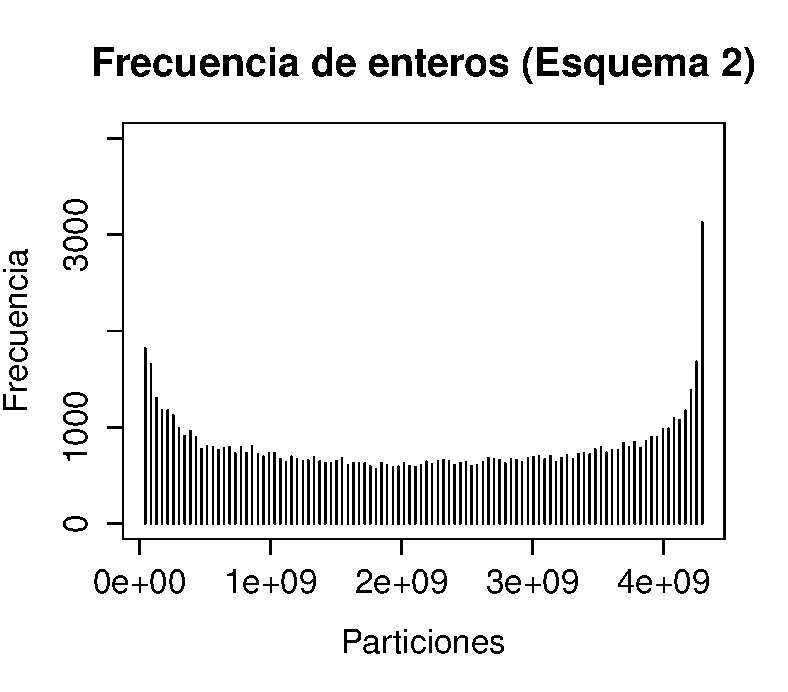
\includegraphics[width=8cm]{figure4.pdf}
\caption{Histograma de valores caóticos discretizados para el esquema 2.}
\label{f4}
\end{figure}


\section{Esquema 3: \textbf{Ocho mapas acoplados con la operación XOR, valores variables para el parámetro $\lambda$}}
\label{esq3}

Para este esquema, se utilizaron los parámetors indicados en la tabla~\ref{table3}.
\begin{table}[H]
\centering
\scalebox{0.9}{
\begin{tabular}{lllll}
\hline   
\textbf{Mapa} & \textbf{Valor} & \textbf{Parámetro} \\
             & \textbf{Inicial} & \textbf{Utilizado} \\
\hline
\textit{Mapa 1}    & 	0.4057062       &  3.9768    \\
\textit{Mapa 2}    & 	 0.1057062           &	  3.9553   \\
\textit{Mapa 3}    & 	0.8057062            &	  3.9368    \\
\textit{Mapa 4}    & 	0.57062        &	  3.99041   \\
\textit{Mapa 5}    &      0.1          &	  3.9989    \\
\textit{Mapa 6}    &        0.897       &	  3.965    \\
\textit{Mapa 7}    &     0.7062           &	  3.9999    \\
\textit{Mapa 8}    & 	0.62        &	  3.918   \\
\hline
\end{tabular}
}
\caption{Valores para cada uno de los mapas utilizados en el esquema 3.}
\label{table3}
\end{table}

En la figura~\ref{pari} se muestra una gráfica de frecuencias de los datos generados por el sistema de mapas logísticos acoplados del esquema~\ref{esq3}, se ha dividido el intervalo $[0,1)$ en 100 particiones, cada valor generado es clasificado en alguna de las particiones. En la figura~\ref{mama} se observan los datos discretos generados.

\begin{figure}[H]  
\centering
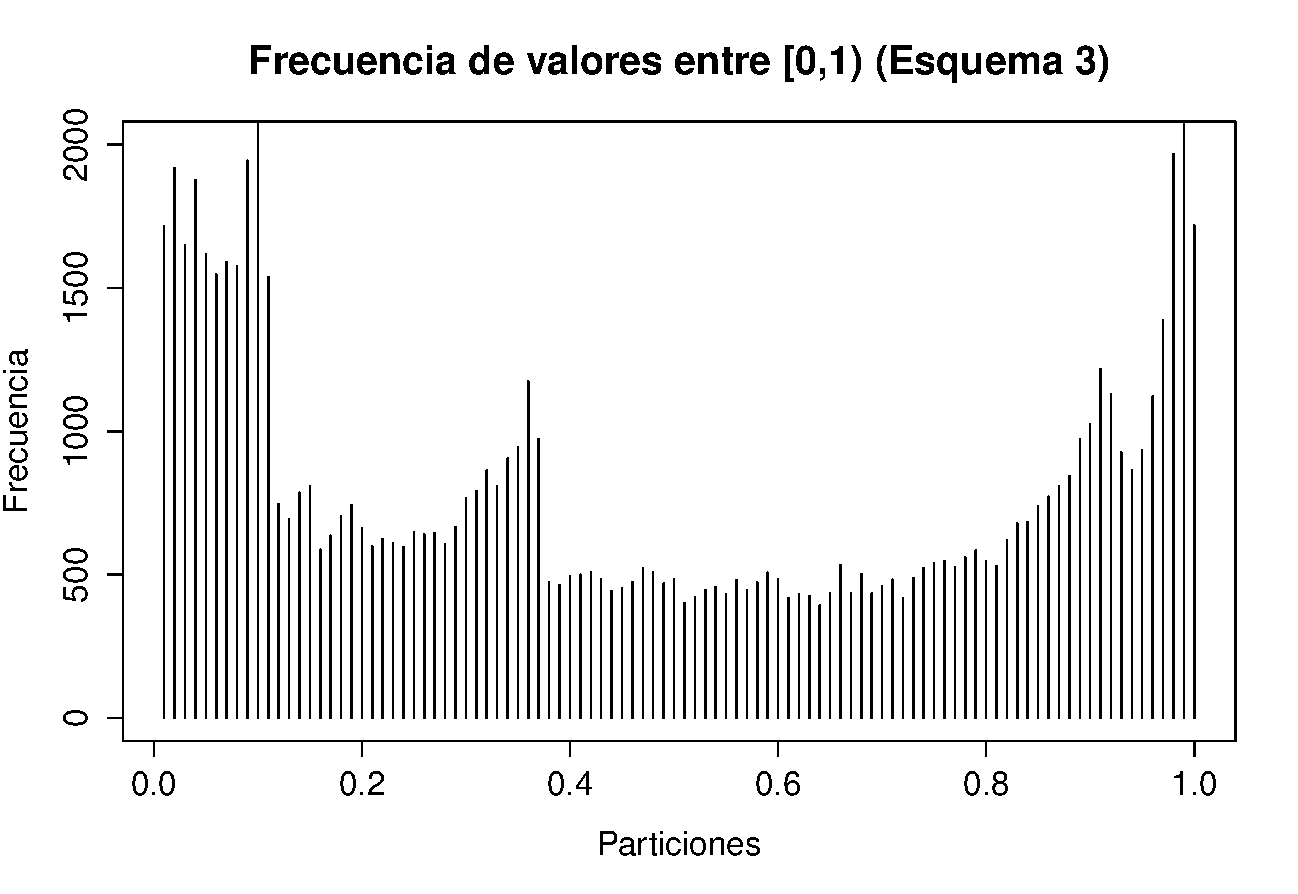
\includegraphics[width=8cm]{fesq3l.pdf}
\caption{Histograma de los valores generados en el esquema 3.}
\label{pari}
\end{figure}


\begin{figure}[H]
\centering
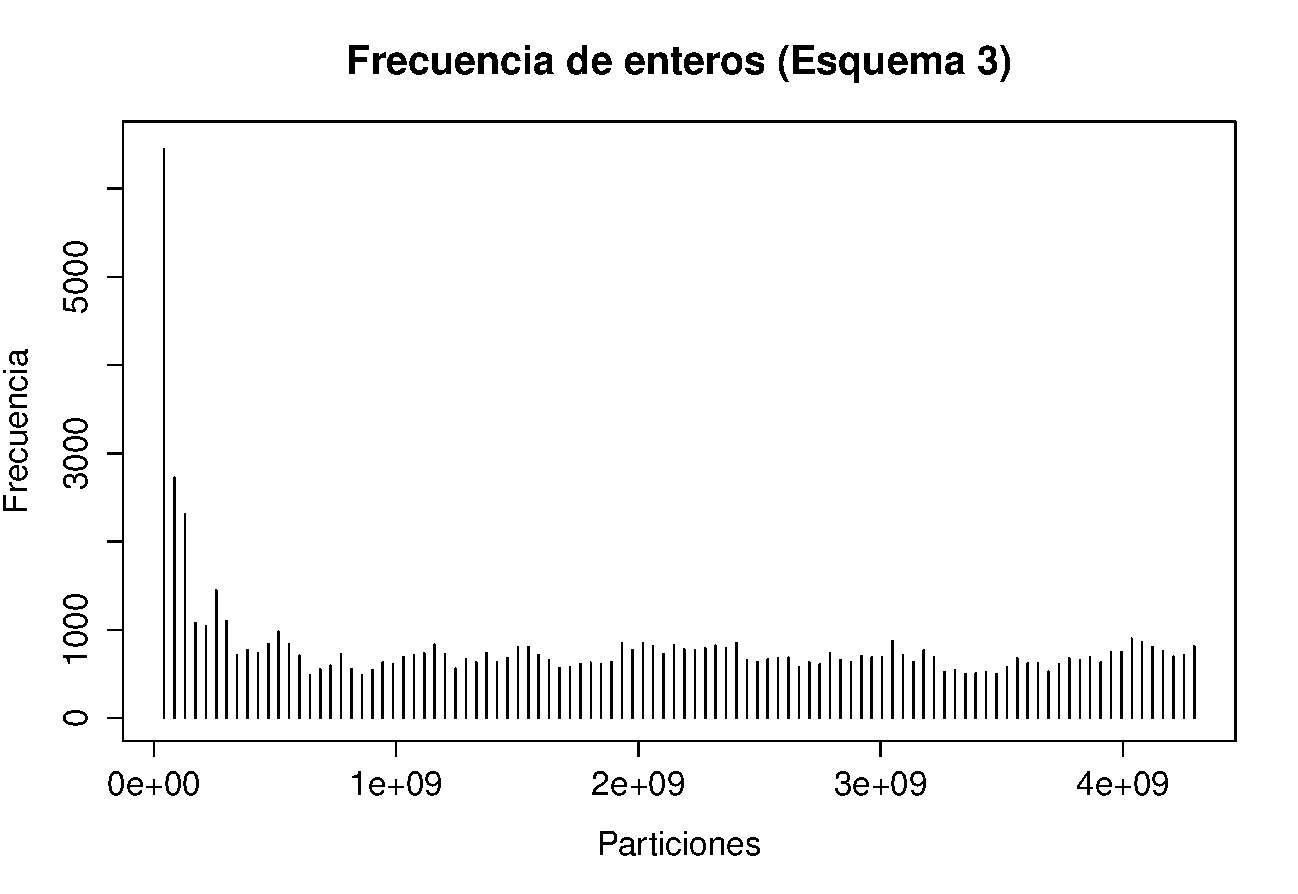
\includegraphics[width=8cm]{cori.pdf}
\caption{Histograma de valores caóticos discretizados para el esquema 3.}
\label{mama}
\end{figure}








\section{Esquema 4: \textbf{Ocho mapas acoplados con la operación XOR, valor constante (3.9999) para el parámetro $\lambda$}}
\label{esq4}

En el esquema 4, se utilizaron los parámetors indicados en la tabla~\ref{table4}.
\begin{table}[H]
\centering
\scalebox{0.9}{
\begin{tabular}{lllll}
\hline   
\textbf{Mapa} & \textbf{Valor} & \textbf{Parámetro} \\
             & \textbf{Inicial} & \textbf{Utilizado} \\
\hline
\textit{Mapa 1}    & 	0.4057062       &     3.9999 \\
\textit{Mapa 2}    & 	 0.1057062      &	  3.9999  \\
\textit{Mapa 3}    & 	0.8057062       &	  3.9999  \\
\textit{Mapa 4}    & 	0.57062         &	  3.9999  \\
\textit{Mapa 5}    &      0.1            &	  3.9999  \\
\textit{Mapa 6}    &        0.897        &	  3.9999  \\
\textit{Mapa 7}    &     0.7062          &	  3.9999  \\
\textit{Mapa 8}    & 	0.62            &	  3.9999  \\
\hline
\end{tabular}
}
\caption{Valores para cada uno de los mapas utilizados en el esquema 4.}
\label{table4}
\end{table}

En la figura~\ref{papa} se muestra una gráfica de frecuencias de los datos generados por el sistema de mapas logísticos acoplados del esquema~\ref{esq4}, se ha dividido el intervalo $[0,1)$ en 100 particiones, cada valor generado es clasificado en alguna de las particiones. En la figura~\ref{tata} se observan los datos discretos generados.

\begin{figure}[H]  
\centering
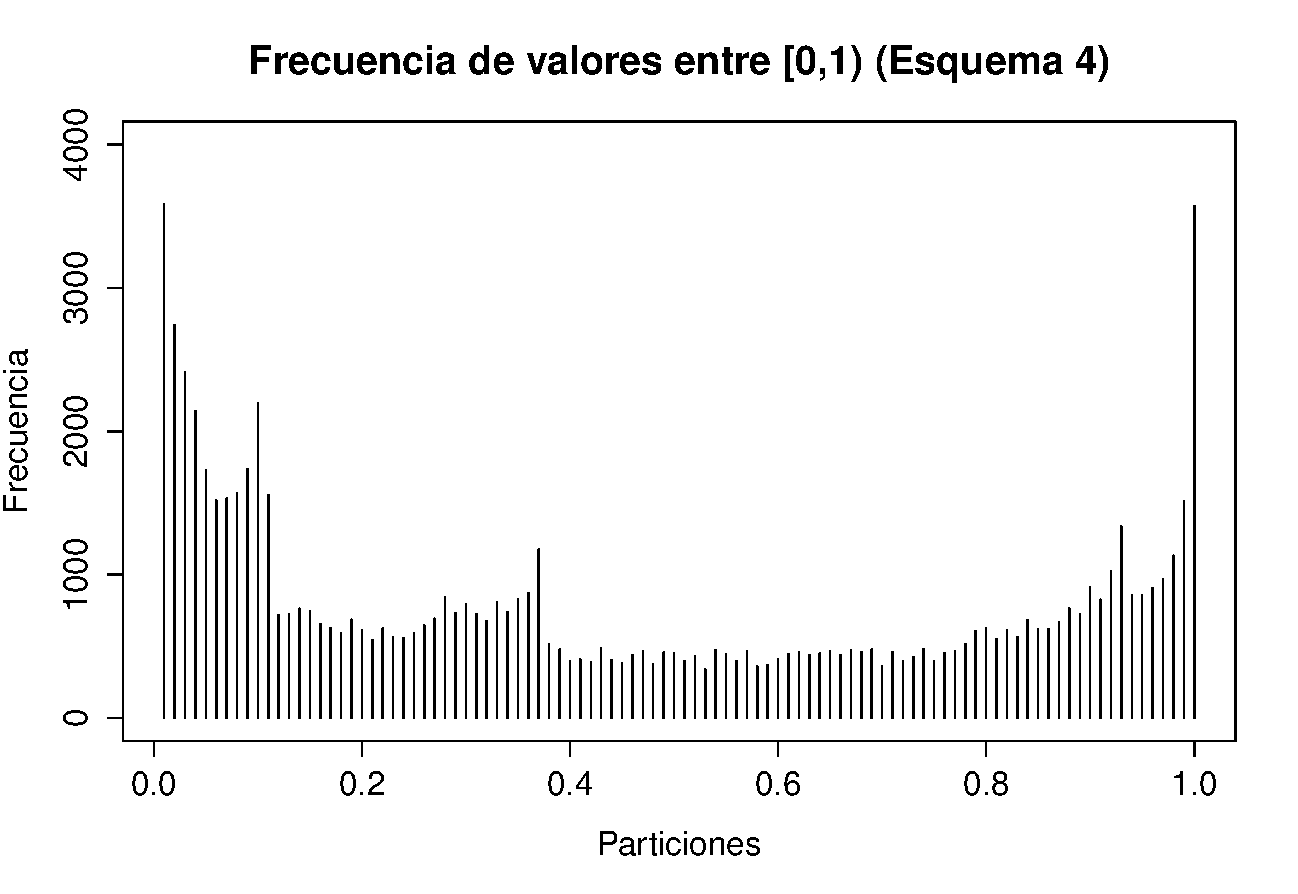
\includegraphics[width=8cm]{papa.pdf}
\caption{Histograma de los valores generados en el esquema 4.}
\label{papa}
\end{figure}


\begin{figure}[H]
\centering
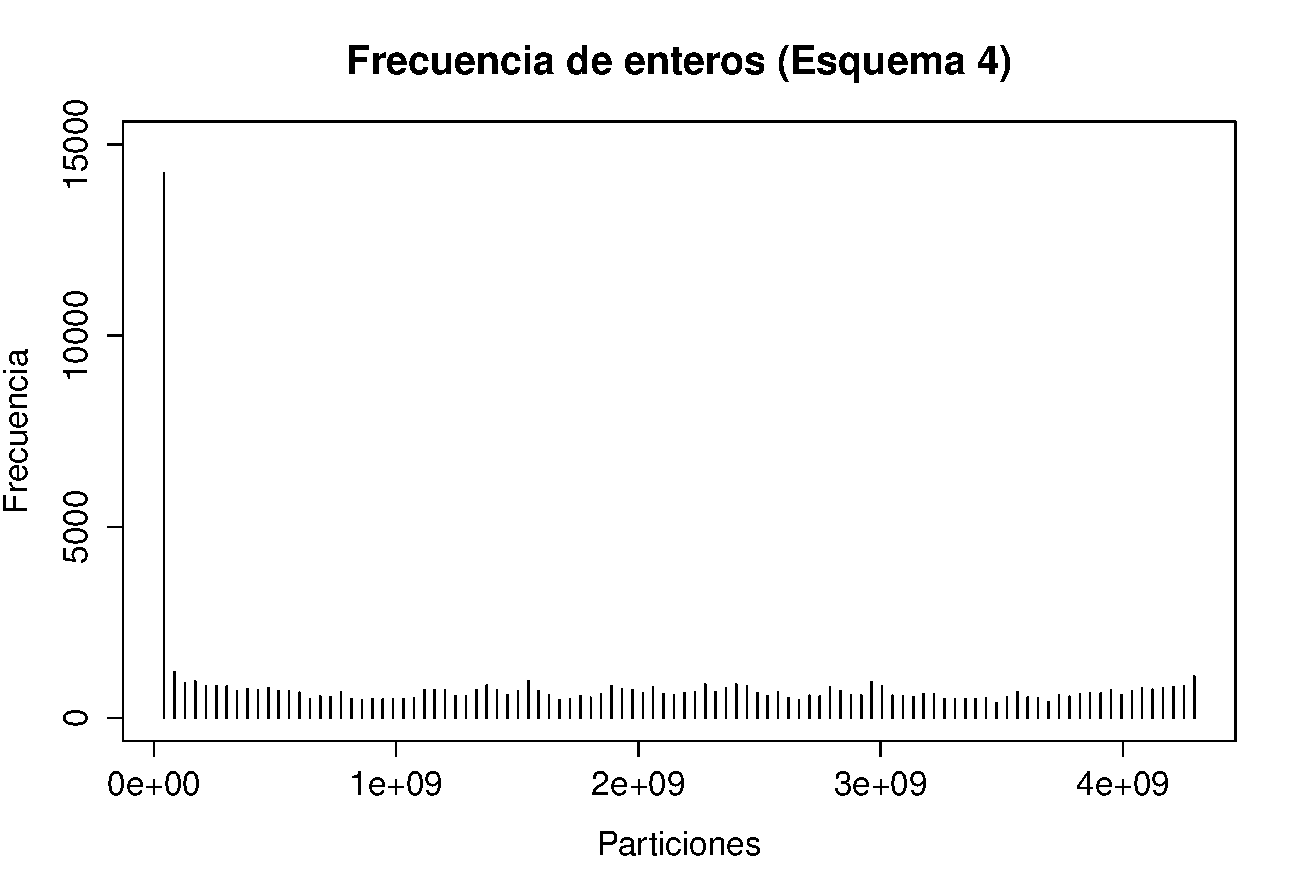
\includegraphics[width=8cm]{tata.pdf}
\caption{Histograma de valores caóticos discretizados para el esquema 4.}
\label{tata}
\end{figure}















\section{Esquema 5: Distintos esquemas con modificaciones.}
\label{esq5}

\subsection{Esquema A}
Este esquema es muy parecido al esquema original, sólo cambia un poco a la hora de aplicar la operación XOR: el contador aumenta en uno. La distribucion de los valores obtenidos se muestran en la figura~\ref{fal} y en la figura~\ref{fad}.



\begin{figure}[H]  
\centering
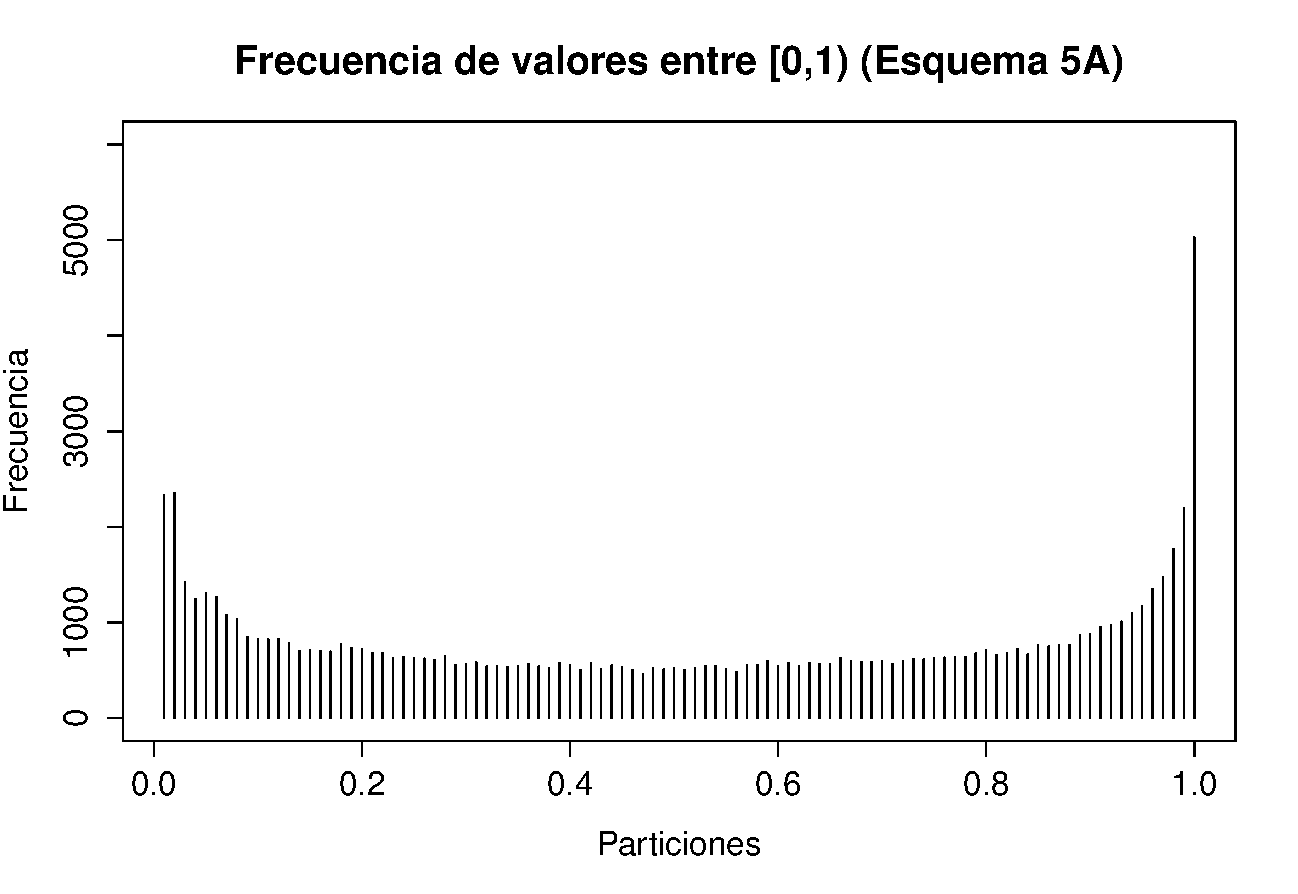
\includegraphics[width=8cm]{faa.pdf}
\caption{Histograma de los valores generados en el esquema 5A.}
\label{fal}
\end{figure}


\begin{figure}[H]
\centering
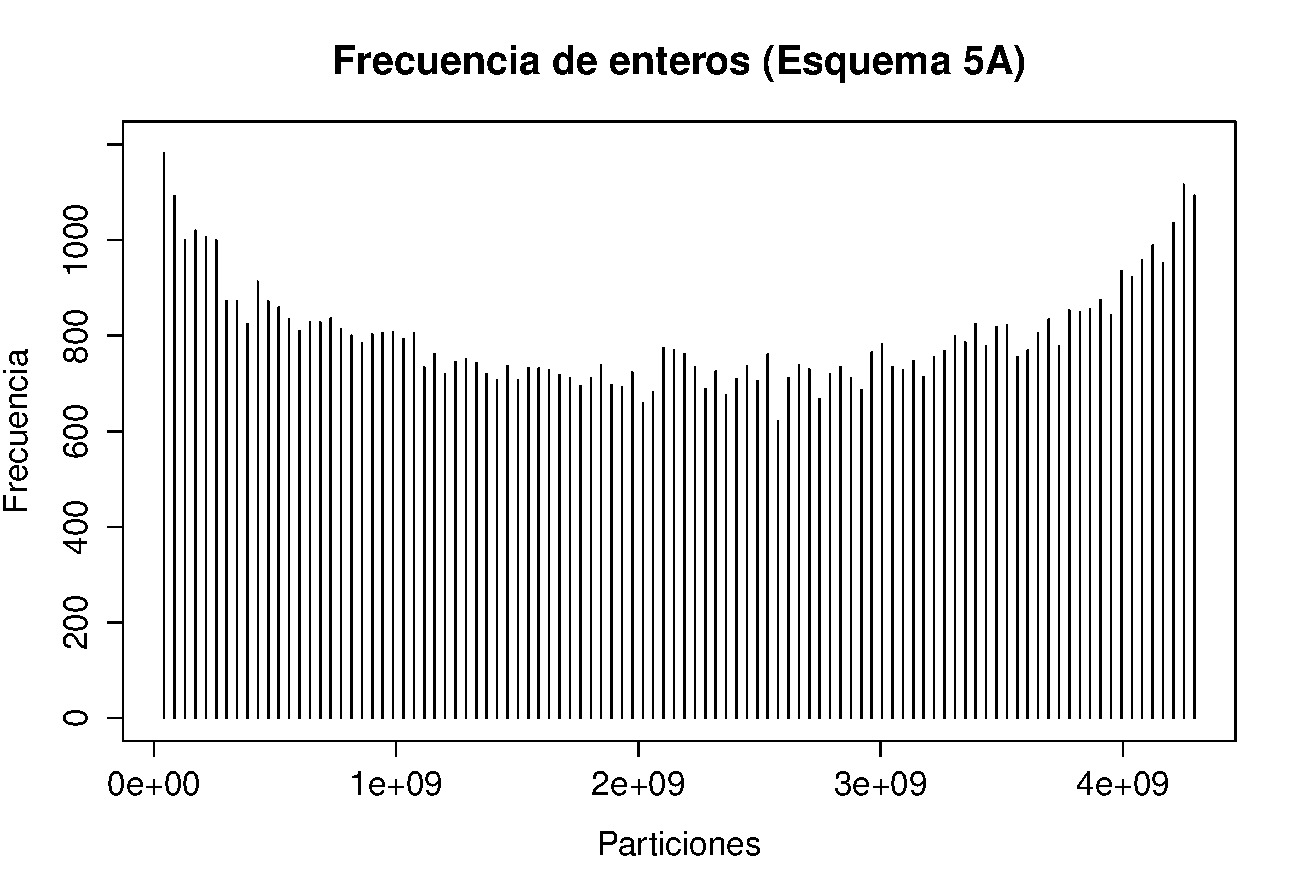
\includegraphics[width=8cm]{fab.pdf}
\caption{Histograma de valores caóticos discretizados para el esquema 5A.}
\label{fad}
\end{figure}




\subsection{Esquema B}
Este esquema también es parecido al esquema original, pero ahora cambia más la manera en cómo se aplica la operación XOR: el contador aumenta en uno; además, se aplica la operación XOR dos veces: la primera vez es un recorrido de izquierda a derecha, la segunda vez es un recorrido de derecha a izquierda. La distribucion de los valores obtenidos se muestran en la figura~\ref{fbl} y en la figura~\ref{fbd}.



\begin{figure}[H]  
\centering
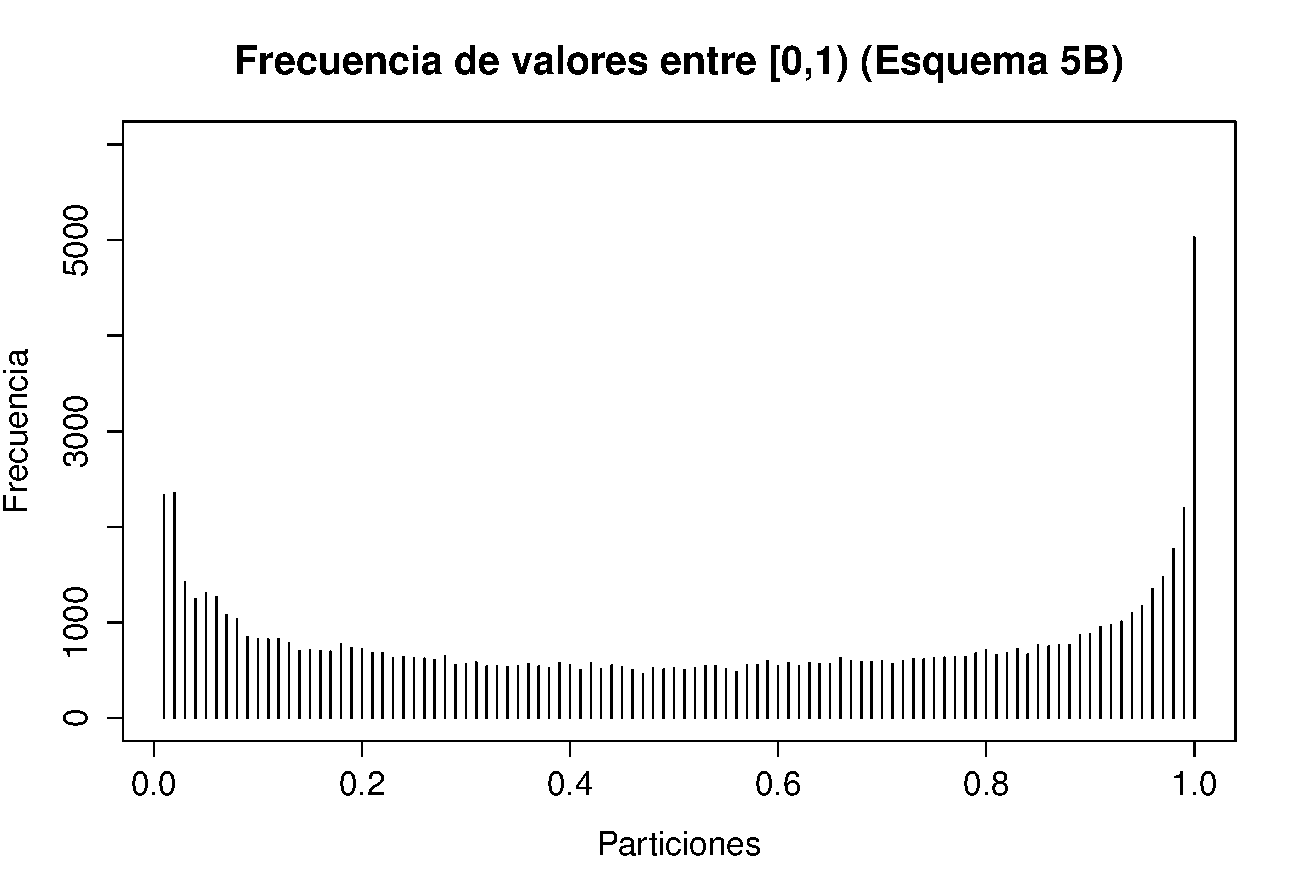
\includegraphics[width=8cm]{fbl.pdf}
\caption{Histograma de los valores generados en el esquema 5B.}
\label{fbl}
\end{figure}


\begin{figure}[H]
\centering
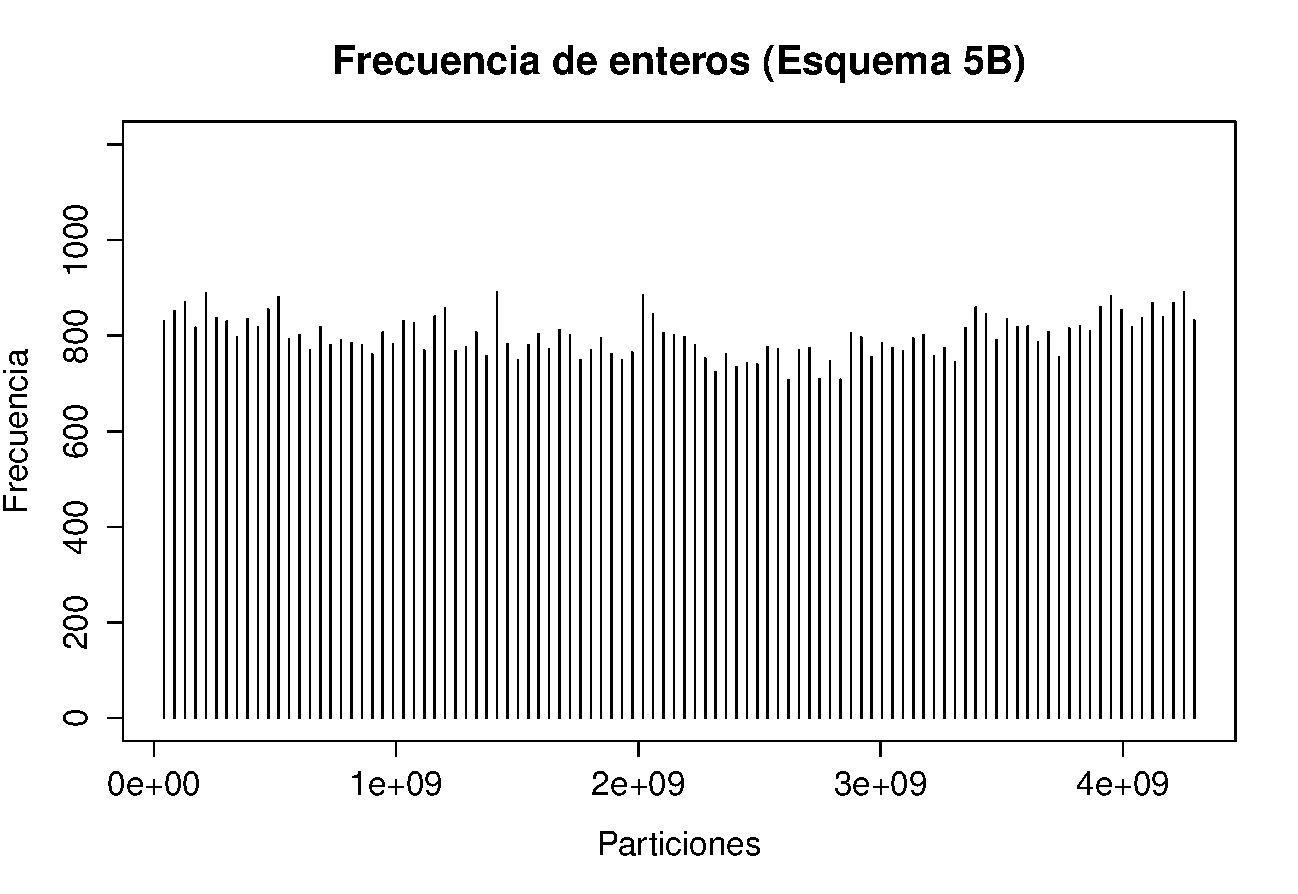
\includegraphics[width=8cm]{fbd.pdf}
\caption{Histograma de valores caóticos discretizados para el esquema 5B.}
\label{fbd}
\end{figure}








\section*{References}

\bibliography{mybibfile}

\end{document}